\documentclass[17pt, margin=1in, innermargin=-2.5in, blockverticalspace=-0.27in]{tikzposter}
\geometry{paperwidth=33.11in,paperheight=46.81in} %A0

\linespread{1.05}
\setlength{\parskip}{0.3em}

% \geometry{paperheight=33.11in,paperwidth=23.4in} %A1
\usepackage[utf8]{inputenc}
\usepackage[T2A]{fontenc}
\usepackage[english]{babel}
\usepackage{csquotes}
\usepackage{amsmath}
\usepackage{amsfonts}
\usepackage{amsthm}
\usepackage{amssymb}
\usepackage{mathrsfs}
\usepackage{graphicx}
\usepackage{lipsum}
\usepackage[export]{adjustbox}
\usepackage{enumitem}
\usepackage[backend=biber, style=ieee]{biblatex}

\usepackage{xcolor}
\usepackage[font=normal, labelfont=bf, width=1.3\linewidth]{caption}

\usepackage[skip=0cm, list=true, labelfont=bf]{subcaption}
%\usepackage{floatrow}
\usepackage{fouriernc}
\usepackage{tempora}
\usepackage{mathtools}
%\usepackage[unicode=true,hidelinks]{hyperref}
%\usepackage[fixlanguage]{babelbib}
\usepackage[oldsyntax]{stackengine}
\usepackage{scalerel}
\usepackage{euscript}

\setlength{\abovecaptionskip}{6pt plus 2pt minus 2pt}
\setlength{\belowcaptionskip}{16pt plus 4pt minus 4pt}

\renewcommand{\figurename}{Fig}


% University of Tartu Computer Science Theme for the tikzposter
% package.
% Author: Joonas Puura, joonas.puura@ut.ee

% Adapted from University of Bristol theme by 
        % Author: Nicholas P Baskerivlle
        % adapted by Rene Welch
        
% Last Modified: 2021-01-10

% Colours are based on style book for University of Tartu: http://stiiliraamat.ut.ee/
% -- COLOURS --


% Primary colour UT
\definecolor{MainBlue}{HTML}{2C5696} % Tunnusvärv, Sinine, Pantone 7685
\definecolor{LightBlue}{HTML}{00A6E6} % Põhipaleti täiendvärv, Helesinine, Pantone 2995
\definecolor{DarkBlue}{HTML}{000000} % Põhipaleti täiendvärv, Tumesinine, SPOT 281 
\definecolor{Orange}{HTML}{c35413} % Aktsentvärv, Oranž, Pantone 151

% Additional colors UT
\definecolor{Gray}{HTML}{B1B3B3} % Lisavärv, Hall, Pantone Cool Gray 5

% Blue as percentage
\colorlet{Blue10}{MainBlue!10} % 10%
\colorlet{Blue20}{MainBlue!20} % 20%
\colorlet{Blue30}{MainBlue!30} % 30%
\colorlet{Blue40}{MainBlue!40} % 40%

% Faculty colours
\definecolor{MedPink}{HTML}{E52143}% Medicine, Pantone 192
\definecolor{AHViolet}{HTML}{AE78B1} % Arts and Humanities, Pantone 7440
\definecolor{STGreen}{HTML}{87BC1F} % Science and Technology, Pantone 376
\definecolor{SocOrange}{HTML}{FAA41A} % Social Sciences, Pantone 137

% Other colours
\definecolor{Black}{HTML}{101820} % Pantone Black 6


% tikzposter color palette

\definecolorpalette{UniTartuPalette} {
    \definecolor{colorOne}{named}{white}
    \definecolor{colorTwo}{named}{Black}
    \definecolor{colorThree}{named}{Black}
}

% tikzposter style
\definecolorstyle{UniTartuStyle} {
    \usecolorpalette{UniTartuPalette}
}{
    % background
    \colorlet{backgroundcolor}{white}
    \colorlet{framecolor}{white}
    % title colors
    \colorlet{titlefgcolor}{Black}
    \colorlet{titlebgcolor}{white}
    % block colors
    \colorlet{blocktitlebgcolor}{colorOne}
    \colorlet{blocktitlefgcolor}{Black}
    \colorlet{blockbodybgcolor}{white}
    \colorlet{blockbodyfgcolor}{Black}
    % innerblock colors
    \colorlet{innerblocktitlebgcolor}{Black}
    \colorlet{innerblocktitlefgcolor}{Black}
    \colorlet{innerblockbodybgcolor}{colorTwo}
    \colorlet{innerblockbodyfgcolor}{Black}
    % note colors
    \colorlet{notefgcolor}{Black}
    \colorlet{notebgcolor}{colorTwo}
    \colorlet{noteframecolor}{colorTwo}
}

% -- STYLE --

% background
\definebackgroundstyle{UniTartuBackgroundStyle}{
    \draw[line width=0pt, color=framecolor, fill=backgroundcolor]
    (bottomleft) rectangle (topright);
}

% title
\definetitlestyle{UniTartuTitleStyle}{
    width=\textwidth, linewidth=2pt, titletotopverticalspace=0in
}{
    \begin{scope}[line width=\titlelinewidth,]
    \draw[color=colorThree,round cap-round cap]
    (\titleposleft,\titleposbottom)--(\titleposright,\titleposbottom);
    \end{scope}
}

% block
\defineblockstyle{UniTartuBlockStyle}{
    titlewidthscale=1.0, bodywidthscale=1.0, roundedcorners=5
}{
    \draw[color=framecolor, fill=blockbodybgcolor,
    rounded corners=\blockroundedcorners] (blockbody.south west)
    rectangle (blockbody.north east);
    \ifBlockHasTitle
    \draw[color=framecolor, fill=blocktitlebgcolor,
    rounded corners=\blockroundedcorners] (blocktitle.south west)
    rectangle (blocktitle.north east);
    \fi
}

% -- THEME -- 
\definelayouttheme{UniTartuTheme}{
    \usecolorstyle[colorPalette=UniTartuPalette]{UniTartuStyle}
    \usebackgroundstyle{UniTartuBackgroundStyle}
    \usetitlestyle{UniTartuTitleStyle}
    \useblockstyle{UniTartuBlockStyle}
    \useinnerblockstyle{Default}
    \usenotestyle{Default}
}

% -- TITLE FORMAT --

% place logo to right of centered title
\makeatletter
\renewcommand\TP@maketitle{%
%   \centering
   \begin{minipage}[b]{0.8\linewidth}
        % \centering
        \color{titlefgcolor}
        {\bfseries \Huge \sc \@title \par}
        \vspace*{1em}
        {\huge \@author \par}
        \vspace*{1em}
        {\LARGE \@institute}
    \end{minipage}%
    \hfill
    \tikz[remember picture,overlay]\node[anchor=south east,xshift=0.42\linewidth,yshift=1cm,inner sep=0pt] {%
        \@titlegraphic
    };
}
\makeatother

%%%%%%%%%%%%%%%%%%%%%%%%%%%%%%%%%%%

\AtBeginEnvironment{tikzfigure}{\captionsetup{type=figure}}

%% ------------------------- %

\newcommand{\shifthat}[2]{%
    \stackengine{\Sstackgap}{$#2$}{\(\hspace{#1}\hat{}\)}{O}{l}{F}{T}{S}
}

% ------------------------- %

\newcommand{\operator}[2][operator]{
    \if H#2\shifthat{0.5em}{#2}\else
    \if d#2\shifthat{0.49em}{#2}\else
    \if q#2\shifthat{0.35em}{#2}\else
    \if \mu#2\shifthat{0.35em}{#2}\else
    \shifthat{0.45em}{#2}
    \fi
    \fi
    \fi
    \fi
}

% ------------------------- %

\newcommand{\vectoperator}[2][operator]{
    \if d#2\shifthat{0.367em}{\textbf{#2}}\else
    \if m#2\shifthat{0.4em}{\textbf{#2}}\else
    \shifthat{0.275em}{\textbf{#2}}
    \fi
    \fi
}

% ------------------------- %

\newcommand{\vect}[3][vector]{
    \overrightarrow{#2_{#3}}
}

% ------------------------- %

\newcommand{\vectbf}[2][bold vector]{
    \vect{\textbf{#2}}
}

% ------------------------- %

\newcommand{\pd}[3][empty]{
    \frac{\partial {#2}}{\partial {#3}}
}

% ------------------------- %

\newcommand{\func}[5][empty]{
    {#2}_{#3}^{#4} \left({#5} \right)
}

% ------------------------- %

\newcommand{\underrel}[3][]{
    \mathrel{\mathop{#3}\limits_{
        \ifx c#1\relax\mathclap{#2}\else#2\fi
    }}
}
%% ------------------------- %

\makeatletter

\newcommand{\Autoref}[1]{\@first@ref#1,@}
\def\@throw@dot#1.#2@{#1}% discard everything after the dot
\def\@set@refname#1{%    % set \@refname to autoefname+s using \getrefbykeydefault
    \edef\@tmp{\getrefbykeydefault{#1}{anchor}{}}%
    \xdef\@tmp{\expandafter\@throw@dot\@tmp.@}%
    \ltx@IfUndefined{\@tmp autorefnameplural}%
        {\def\@refname{\@nameuse{\@tmp autorefname}}}%
        {\def\@refname{\@nameuse{\@tmp autorefnameplural}}}%
}
\def\@first@ref#1,#2{%
\ifx#2@\autoref{#1}\let\@nextref\@gobble% only one ref, revert to normal \autoref
\else%
    \@set@refname{#1}%  set \@refname to autoref name
    \@refname\ref{#1}% add autoefname and first reference
    \let\@nextref\@next@ref% push processing to \@next@ref
\fi%
\@nextref#2%
}
\def\@next@ref#1,#2{%
\ifx#2@,~\ref{#1}\let\@nextref\@gobble% at end: print and+\ref and stop
\else, \ref{#1}% print  ,+\ref and continue
\fi%
\@nextref#2%
}

\makeatother

% ------------------------- %
%% ------------------------- %

\newcommand{\img}[4][anything]{
    \begin{figure}[H]{
        \center{\includegraphics[width={#4}]{{#1}}}
        \caption{#2}\label{#3}}
    \end{figure}
}

% ------------------------- %

\newcommand{\floatimg}[4][anything]{
    \begin{figure}[ht]{
        \center{\includegraphics[width={#4}]{{#1}}}
        \caption{#2}\label{#3}}
    \end{figure}
}

% ------------------------- %

\newcommand{\subimg}[2][anything]{
    \begin{minipage}[h]{{#2}} % 0.4\textwidth
        \center{\includegraphics[width=1\linewidth]{{#1}}}
    \end{minipage}
}

% ------------------------- %

\newcommand{\subimgtwo}[4][anything]{
    \subfloat[{#2}]{\includegraphics[width={#4}]{{#1}}\label{#3}}
}

% ------------------------- %
%\newsavebox{\foobox}

\newcommand{\slantbox}[2][0]{\colorlet{slantcolor}{.}\mbox{%
        \sbox{\foobox}{\color{slantcolor}#2}%
        \hskip\wd\foobox
        \pdfsave
        \pdfsetmatrix{1 0 #1 1}%
        \llap{\usebox{\foobox}}%
        \pdfrestore
}}
\newcommand\unslant[2][-.2]{%
  \mkern1mu%
  \ThisStyle{\slantbox[#1]{$\SavedStyle#2$}}%
  \mkern-1mu%
}
\newcommand\upmu{\unslant\mu}

%%%%%%%%%%%%%%%%%%%%%%%%%%%%%%%%%%%

\makeatletter
\setlength{\TP@visibletextwidth}{31.0in}
\setlength{ \TP@visibletextheight}{45in}
\makeatother
\usepackage{mwe} % for placeholder images
\usepackage{bm}
\usepackage{bbm}



% set theme parameters
\tikzposterlatexaffectionproofoff
\usetheme{UniTartuTheme}
\usecolorstyle{UniTartuStyle}
% ------------------------- %

\newcommand{\shifthat}[2]{%
    \stackengine{\Sstackgap}{$#2$}{\(\hspace{#1}\hat{}\)}{O}{l}{F}{T}{S}
}

% ------------------------- %

\newcommand{\operator}[2][operator]{
    \if H#2\shifthat{0.5em}{#2}\else
    \if d#2\shifthat{0.49em}{#2}\else
    \if q#2\shifthat{0.35em}{#2}\else
    \if \mu#2\shifthat{0.35em}{#2}\else
    \shifthat{0.45em}{#2}
    \fi
    \fi
    \fi
    \fi
}

% ------------------------- %

\newcommand{\vectoperator}[2][operator]{
    \if d#2\shifthat{0.367em}{\textbf{#2}}\else
    \if m#2\shifthat{0.4em}{\textbf{#2}}\else
    \shifthat{0.275em}{\textbf{#2}}
    \fi
    \fi
}

% ------------------------- %

\newcommand{\vect}[3][vector]{
    \overrightarrow{#2_{#3}}
}

% ------------------------- %

\newcommand{\vectbf}[2][bold vector]{
    \vect{\textbf{#2}}
}

% ------------------------- %

\newcommand{\pd}[3][empty]{
    \frac{\partial {#2}}{\partial {#3}}
}

% ------------------------- %

\newcommand{\func}[5][empty]{
    {#2}_{#3}^{#4} \left({#5} \right)
}

% ------------------------- %

\newcommand{\underrel}[3][]{
    \mathrel{\mathop{#3}\limits_{
        \ifx c#1\relax\mathclap{#2}\else#2\fi
    }}
}

%\usepackage[scaled]{helvet}
%\renewcommand\familydefault{\sfdefault} 
%\renewcommand{\vec}[1]{\bm{#1}}
%\newcommand{\Tr}{\text{Tr}}

\addbibresource{refs.bib}
\addbibresource{components/bibliography.bib}

\title{\parbox{0.8\linewidth}{Angular dispersion boost of high order laser harmonics interacting with dense plasma clusters}}
\author{\textbf{L.A. Litvinov}\textsuperscript{1}, \textbf{A.A. Andreev}\textsuperscript{1, 2}}
\institute{\textsuperscript{1}\textit{Saint Petersburg State University, Saint Petersburg, Russia} \\ \textsuperscript{2}\textit{Ioffe Physico-Technical Institute, Saint Petersburg, Russia}}

%\titlegraphic{
\includegraphics[width=0.06\linewidth]{../components/img/spbu_logo2.png}}

% begin document
\begin{document}
    \maketitle
    \centering
    \begin{columns}
        \column{0.33}

        \block{}{
            It is well known the interaction of intense coherent radiation with limited size targets can cause the excitation of surface plasmon oscillations. Absorption and scattering of the incident light in such case can be described good enough using the Mie theory, which predicts the multipole resonances corresponding to oscillations of a part of free electrons of the target with respect to positively charged ions. In this mode, effective excitation of surface plasmons can cause a significant increase
internal and external fields at eigenfrequencies, for example, gas os clusters, as well as the enhancement of scattered field at large angles with respect to the incident wave direction.

Mirrors and diffraction gratings can be used to manage spatial characteristics of the infrared and visible wavelength range. On the other side, crystals with regularly spaced scattering centers are suitable for X-ray radiation direction. However, there is a large gap between these wavelength ranges, hard or extreme ultraviolet radiation (XUV), corresponding to high-order laser harmonics in particular. XUV light turns out to be difficult to control due to high absorption of any material in this range.

\begin{figure}[H]
    \subimgtwo[components/img/celes/TE_10deg_check]{$\theta = 10^{\circ}$. Efficient scattering at angles $
    \theta_{\textrm{s}} = 0^{\circ}$, $-24^{\circ}$, $135^{\circ}$ with respect to the incidence direction.}{fig:a}{0.48\textwidth}
    \hfil
    \subimgtwo[components/img/celes/TE_15deg_check]{$\theta = 15^{\circ}$. Efficient scattering at angles $
    \theta_{\textrm{s}} = 0^{\circ}$, $-27^{\circ}$ with respect to the incidence direction.}{fig:b}{0.48\textwidth}
    \caption{10-th harmonic scattering by cubic lattice of clusters $12\times12\times12$. $\theta$ is the angle of lattice rotation around $y$ axis (equals to different incident light angles). $|\vectbf{E}{\textrm{s}}|$ plotted in the plane perpendicular to polarizaiton: $\vectbf{e}{\textrm{p}} = \vectbf{e}{y}$. Incident radiation represented by the gaussian beam with width $w = 300$ nm.}
    \label{fig:image}
\end{figure}

In this work we propose usage of a medium of spherical nano-clusters as a target for efficient directed scattering radiation in the XUV range. It was shown, with the linear Mie scattering theory, it is possible to estimate the resonance parameters of a single cluster and predict potential scattering directions for a system of many clusters.

Using a cubic lattice spatial configuration, options for diffraction control of 10-th titan-sapphire laser harmonic were calculated and the features of scattering with respect to the angle incidence of radiation were revealed (\autoref{fig:image}). The results show the correspondence of the Bragg-Wolfe diffraction theory for planar and spatial gratings, the ability to control high harmonics of laser radiation (XUV range) using an ionized cluster gas.

        }

        \block[bodyoffsety=0.7cm]{Introduction}{
            \setlength{\parindent}{1em}
            \section{Introduction}

Limited size targets interacting with high-intensity coherent radiation is well-studied phenomenon of linear excited surface plasmonic oscillations. Absorption and scattering of incident light in this case good described with Mie theory predicting exist of resonance corresponding to multipole oscillations of part of the target free electrons relative to positive charged ions. In resonance mode efficient exciting of surface plasmons can lead to significant boost internal and external field on fundamental cluster frequency (eigenfrequency). In turn, this can cause enhancement of field scattered on large angles relative to the direction of incident wave. 

In micrometer wavelengths photon crystals and lattices can be used for direction or diffraction electromagnetic waves~\cite{lin_zhang}, while for x-ray radiation it is possible to use real crystals with regularly placed scattering centers (atoms) with distance of few nanometers~\cite{batterman_cole}. At the same time, large interval between these wavelength orders named XUV (extreme-ultraviolet) is hard to manipulate.

Within the present work we consider the possibility of directed scattering of short wavelength radiation in the XUV range by scattering on suitable spherical clusters. Similar case with cylindrical symmetry (arrays of nanocylinders as scatterers) was researched earlier~\cite{andreev_lecz}. Of course, nanocylinders are more suitable regarding the control of size an distance parameters at the target manufacturing stage, but arrays of spherical clusters can make possible to manipulate with light direction in three-dimensional space and give a more optimal spatial configuration.

\img[components/img/gas_cluster4]{Clusters generation process by adiabatic expansion of gas.}{cluster_gas_sheme:image}{}{0.7\textwidth}

It is known that a short intense laser pulse can generate high-order harmonics by interacting with dense solid surfaces. But intensity of high-order harmonics generated in gases is at least 4 orders of magnitude less that is not enough to ionize the target and generate a plasma with fully imaginary refractive index that we need --- in our case, spherical clusters are ionized cluster gas (\autoref{cluster_gas_sheme:image}). To solve this problem we propose to use intense preceding pulse to pre-ionize the target and reach required plasma generation.

Common interaction scheme is shown in \autoref{plasma_area1:image}. Harmonics in the main pulse have different intensity depending on the angle, that leads to the angle dependence of output radiance shape. The scattering by a single cluster can be completely described in spherical symmetry and the interaction can be easily modeled with the help of particle in cell simulations. We propose to use linear approximation by Mie theory as assessment for further modeling. In general, we concentrate on a theoretical investigation, supported by simulations, and we point out the applicability for experimental realisation.

\img[components/img/plasma_area2]{Interaction scheme. The plane of polarization is parallel to one of the faces of cubic region. The dimensions of spherical clusters are about a few nanometers, distance between them is at least wavelength. In general, the distribution of clusters within a cubic region is random, clusters do not intersect the edges of the region and each other.}{plasma_area1:image}{}{0.8\textwidth}

        }

        \block[bodyoffsety=0.7cm]{Analytical model}{
            \setlength{\parindent}{1em}
            \section{Base model}

Let us consider a single cluster with radius $a$ irradiated by short femtosecond pulse with intensity about $I_{h} \approx 10^{14}$ $\textrm{W/cm}^2$. The Drude model yields the dielectric function of the plasma:

    \eq
		\varepsilon (\w) = 1 - \left( \frac{\w_{pe}}{\w} \right)^2 \frac{1}{1 + i \beta_{e}}, \qquad \w_{pe} = \sqrt{\frac{4 \pi e^2 n_e}{m_e}},
		\label{eps_plasma}
	\qe

\noindent where $\w$ --- harmonic (angular) frequency under consideration; $\w_{pe}$ --- the electron plasma frequency; $e$, $m_e$ --- electron charge and mass; $n_e = Z n_i$ --- the electron number density, where $Z$ --- average ionization degree, $n_i$ --- ion density. $\beta_{e} = v_e / \w$ and $v_e$ --- electron-ion collision rate in Spitzer approximation. As we are going to consider scattering of harmonic radiation, the cluster should have a density above the critical one for this harmonic: $n_c = \w^2 m_e / 4 \pi e^2$. Thus for example, for 10-th laser harmonic with wavelength $\lambda_{L} = 830$ nm one obtains condition $n_e > 1.3 \cdot 10^{23}$ $\textrm{cm}^{-3}$.

The Mie theory can be used for the description of elastic electromagnetic wave scattering by arbitrary sized particles in case of linear interactions and let obtain scattered and internal field. A main step is to solve the scalar Helmholtz Equation in suitable coordinate system andgain the vector solutions. For spherical cluster the solution of corresponding equation can be written in the form of Bessel and Hankel functions of $n$-th order~\cite{boren_huffman}.

Assume an incident plane wave propagating along $z$ axis of cartesian coordinate system and polarized along $x$ axis:

    \eq
        \vectbf{E}{i} = E_0\:e^{i\w t - ikz}\:\vectbf{e}{x},
        \label{E_i_sph}
    \qe

\noindent where $k = \w/c$ --- wavenumber, $\vectbf{e}{x}$ --- the unit vector of $x$ axis direction and polarization vector:

    \img[components/img/single_sph_scheme]{Base model scheme.}{single_sph_scheme:image}{0.73\textwidth}

Now we can expand the plane wave into series using generalized Fourier expantions. Assuming our media is isotropic we obtain following form of scattered field~\cite{boren_huffman}:

    \eq
		\vectbf{E}{s} = \sum_{n = 1}^{\infty}E_n \left[ i a_n\left(ka, m\right) \vectbf{N}{}^{(3)}_{e1n} - b_n\left(ka, m\right) \vectbf{M}{}^{(3)}_{o1n} \right], \qquad E_n = i^{n} E_0 \frac{2n + 1}{n \left( n + 1\right)}
        \label{E_s_sph}
	\qe

$n$ --- vector harmonic number after cartesian-spherical coordinate system transformation, $m = \sqrt{\varepsilon\left(\w\right)}$ --- refractive index of the target. Vector harmonics coefficients have the following form~\cite{boren_huffman}:


    \eq
		a_n(x,\:m) = \frac{m \func{\psi}{n}{\prime}{x} \func{\psi}{n}{}{mx} - \func{\psi}{n}{\prime}{mx} \func{\psi}{n}{}{x}}{m \func{\xi}{n}{\prime}{x} \func{\psi}{n}{}{mx} - \func{\psi}{n}{\prime}{mx} \func{\xi}{n}{}{x}},
		\label{an_bessel}
	\qe

    \eq
        b_n(x,\:m) = \frac{\func{\psi}{n}{\prime}{x} \func{\psi}{n}{}{mx} - m \func{\psi}{n}{\prime}{mx} \func{\psi}{n}{}{x}}{\func{\xi}{n}{\prime}{x} \func{\psi}{n}{}{mx} - m \func{\psi}{n}{\prime}{mx} \func{\xi}{n}{}{x}},
        \label{bn_bessel}
    \qe
    \eqc % artificial indent after the equation
    \cqe %

\noindent $\func{\psi}{n}{}{z} = z \func{j}{n}{}{z}$, $\func{\xi}{n}{}{z} = z \func{h}{n}{}{z}$ --- Riccati-Bessel functions, $h_n = j_n + i \gamma_n$ --- spherical Hankel functions of the first kind. 

In case of spherical symmetry amplitude of the scattered field is maximum for $m^2 = - (n+ 1) / n$ when $ka \ll 1$, that gain corresponding set of resonance densities in collision-less case: $n_e = n_c(2n + 1) / n$. It can be obtained using zero-order (asymptotic) approximation of Bessel functions, after which coefficients (\Autoref{an_bessel, bn_bessel}) are significant simplified:

    \eq
        a_n\left( x \to 0,\:m \right) = \left( 1 + 2i \frac{ (2n - 1)! (2n + 1)!}{4^n \: n! (n + 1)!} \frac{\left(m^2 + \frac{n + 1}{n} \right)}{(m^2 - 1)} \frac{1}{x^{2n+1}} \right)^{-1}, \qquad b_n\left( x \to 0,\:m \right) = 0
        \label{ab_asymp}
    \qe

This approximation can be used instead of (\Autoref{an_bessel, bn_bessel}) for scatterers with quite small radius, but for $ka \sim 1$ the approximation ceases to be reasonable already, particularly for large $n$. Instead, in this case, the first-order approximation is better suited:

    \eq
		a_n\left( x ,\:m \right) = \left( 1 + i \frac{ C_n x^{-1 -2n} \left( (4(1 + n + m^2 n) (-3 + 4n (1 + n)) - 2(m^2 - 1)(3 + n(5 + 2n + m^2 (2n - 1))) x^2) \right)}{\pi (m^2 - 1)(2n + 3)(n + 1)(4(2n + 3) - 2(m^2 + 1)x^2)} \right)^{-1}
		\label{an_sph_asymp1}
	\qe
	\eqc
		C_n = 2^{1 + 2n} \Gamma(n - \frac{1}{2}) \Gamma(n + \frac{5}{2})
	\cqe

\autoref{ab_asymp:image} shows dependence of the scattering coefficient on the electron density for two different values of the radius in zero-order approximation. We can compare it with the first-order for $ka = 1.5$ (\autoref{ab1:image}). We can see, that with increase of $n$ width of the resonance peak decreases rapidly. Larger $ka$ corresponds to larger peak width. Besides that, with increase of $ka$ value of the resonance density increases, that shown in \autoref{nenc_123:image}.

    \begin{figure}[H]
        \subimgtwo[components/img/sph_base/sph_ka0.5_123]{$ka = 0.5$.}{ab_asymp:a}{0.66\textwidth}\\
        \subimgtwo[components/img/sph_base/sph_ka1.5_123]{$ka = 1.5$.}{ab_asymp:b}{0.66\textwidth}
		\caption{Spherical harmonics coefficients in zero-order approximation, $\beta_e = 0$. "Exact" curves were plotted using full expansions of the Bessel and Hankel fucntions.}
		\label{ab_asymp:image}
	\end{figure}

    \img[components/img/sph_base/sph_ka1.5_123_1st]{$ka = 1.5$ in first-order approximation. $\beta_e = 0$. "Exact" curves were plotted using full expansions of the Bessel and Hankel fucntions.}{ab1:image}{0.66\textwidth}

Such approximations allow us to estimate the resonance cases for a material with pre-defined refractive index $m$ as well as estimate refractive index corresponding to the required wavelength. As we consider XUV range radiation (20-120 nm), radiuses of spherical scatterers should be about few nanometers, that causes $ka \sim 1$. Obviously, for such $ ka $ the resonance values of the electron density can be large in considering $n = 1$ as term with the largest contribution to the scattered field. Staying within high-temperature plasma we should use only $n_e < 10^{24}$ $\textrm{cm}^{-3}$. Thus for $ka > 0.9$ it is more reasonable to estimate the resonance electon density using $n = 2$.

Using first-order approximation (\ref{an_sph_asymp1}) with wavelength $\lambda_{10} = \lambda_{L} / 10 = 83$ nm we get $n_e \approx 5 \cdot 10^{23}$ $\textrm{cm}^{-3}$ for $ka \approx 0.5$ and $n_e \approx 5.7 \cdot 10^{23}$ $\textrm{cm}^{-3}$ for $ka \approx 0.7$ to reach efficient scattering.

    \img[components/img/sph_base/nenc_123]{Resonance electron density depending on radius. Curves were calculated in maximum points of (\ref{an_sph_asymp1}), $\beta_e = 0$.}{nenc_123:image}{0.66\textwidth}




        }

        \column{0.33}

        \block[bodyoffsety=0.7cm]{}{
            \setlength{\parindent}{1em}
            Using approximations of the Bessel functions~\cite{boren_huffman} we can significantly simplify the coefficients (\ref{an_bessel},~\ref{bn_bessel}) and obtain resonance conditions for the electon density and cluster radius. 

% Such approximations can be used instead of the exact equations for objects of $ka \ll 1$, but for $ka \sim 1$ and larger higher-order approximations obtained in a similar way~\cite{boren_huffman} are suitable (Fig.~\ref{ab_asymp:image}).

%  Such approximations make it possible to estimate the resonance parameters of the cluster, in particular, the electron density and radius.
%  Wavelength $\lambda_{10} = \lambda_{L} / 10 = 83$ nm corresponds to the resonant electron density $n_{el} \approx 5.7 \cdot 10^{23}$ $\textrm{cm}^{-3}$ for $ka = 0.7$ and $n_{el} \approx 3.9 \cdot 10^{23}$ $\textrm{cm}^{-3}$ for $ka = 0.3$, with medium ionization degrees $Z|_{ka = 0.7} \approx 9$ and $Z|_{ka = 0.3} \approx 6$.

        }

        \block[bodyoffsety=0.7cm]{Single cluster}{
            \setlength{\parindent}{1em}
            To check the resulting analytical model, we calculated the values of the complex refractive index $m$, which correspond to the previously obtained conditions for the resonance electron density $n_{el}$ at $\lambda_{10} = 83$ nm, $ka = 0.7$: $m = 1.851i$ (\ref{m2_resonance}). The complex refractive index is purely imaginary, since the collision coefficient $v_e$ in the case under consideration is somewhat lower than the harmonic frequency, so the interaction can be considered collisionless~\cite{andreev_lecz}.

For this case, the scattered electric field (\ref{E_s_sph}) was calculated for $\lambda = \lambda_{L}$ and $\lambda = \lambda_{10}$ in order to compare the resonant and nonresonant cases. It can be seen that in the resonance case (\ref{ka0.7:b}) the scattered field is a diverging spherical wave, the field amplitude in the vicinity of the cluster is much higher than in the absence of resonance (\ref{ka0.7:a}), where Scattered waves as such are practically not observed, which indicates that the incident wave in the nonresonant case practically does not interact with the cluster.

    \begin{tikzfigure}
        \subcaptionbox{$\lambda = \lambda_{L} = 830$ nm.}{
            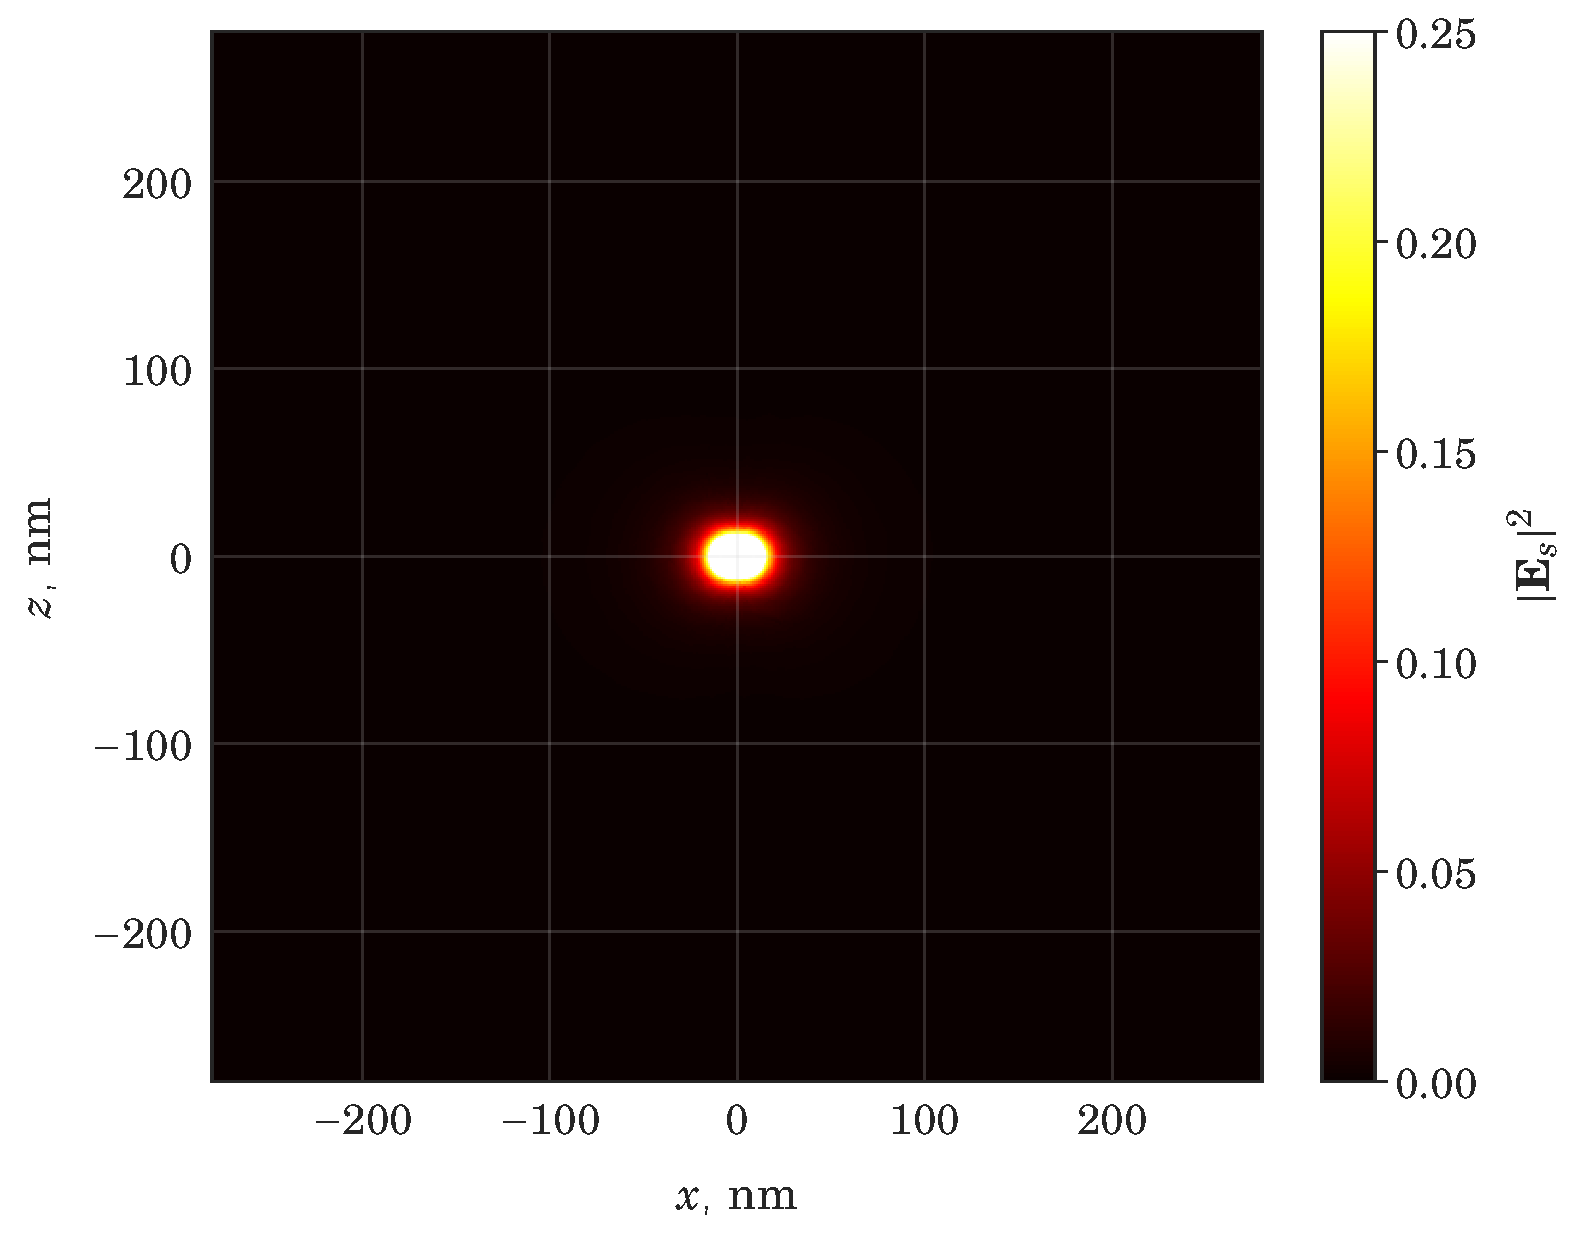
\includegraphics[width=0.45\linewidth]{../components/img/mph_new/es_ka0.7_1harm}
        }
        \hfil
        \subcaptionbox{$\lambda = \lambda_{10} = 83$ nm.}{
            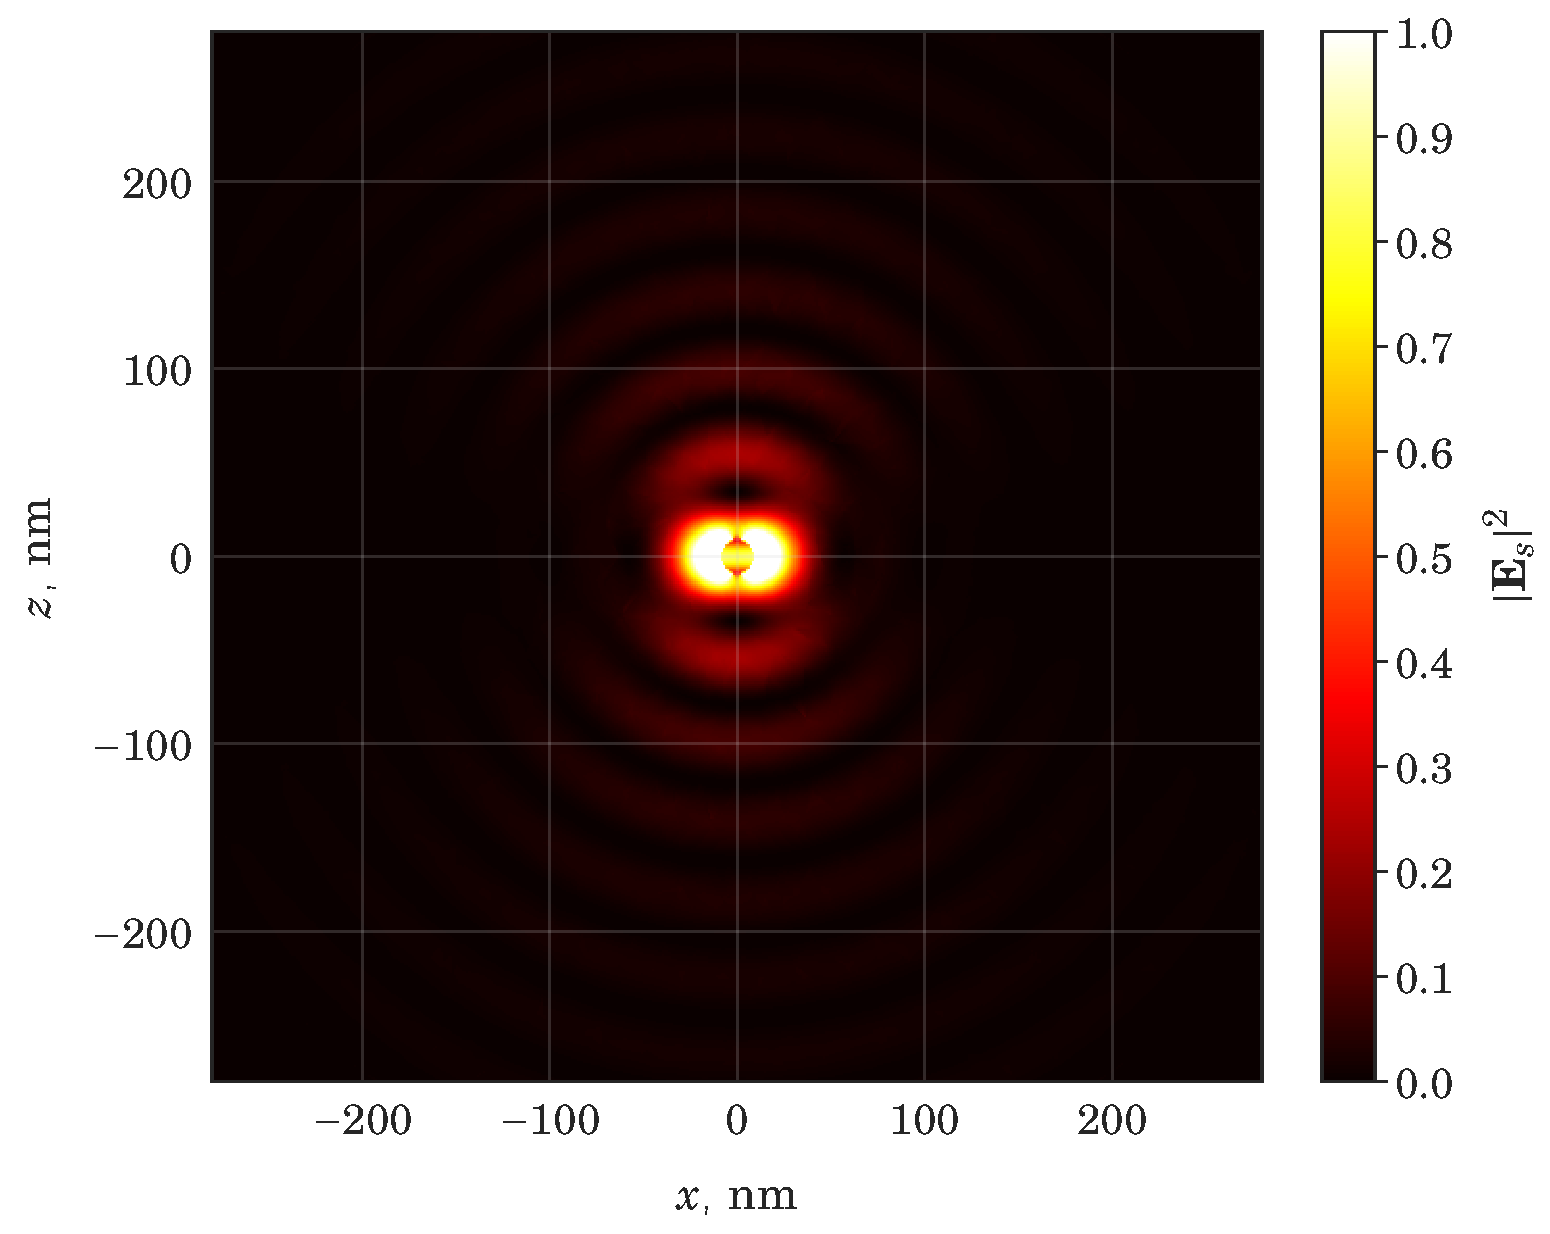
\includegraphics[width=0.45\linewidth]{../components/img/mph_new/es_ka0.7_10harm}
        }
        \label{ka0.7:image}\caption{$ka = 0.7$ ($a \approx 8.9$ nm); $|\vectbf{E}{s}|^2$ in the plane of polarization of the incident wave.}
    \end{tikzfigure}

    % \begin{figure}[H]
    %     \subimgtwo[components/img/mph_new/es_ka0.7_1harm]{$\lambda = \lambda_{L} = 830$ nm.}{ka0.7:a}{0.4\textwidth}
    %     \hfil
    %     \subimgtwo[components/img/mph_new/es_ka0.7_10harm]{$\lambda = \lambda_{10} = 83$ nm.}{ka0.7:b}{0.4\textwidth}
    %     \caption{$ka = 0.7$ ($a \approx 8.9$ nm); $|\vectbf{E}{s}|^2$ в плоскости поляризации падающей волны.}\label{ka0.7:image}
    % \end{figure}

    % \begin{figure}[H]
    %     \subimgtwo[components/img/mph_new/es_ka1.7_10harm]{Рассеяние кластером.}{10h_ka0.7:a}{0.4\textwidth}
    %     \hfil
    %     \subimgtwo[components/img/external/oe-28_screen_single.jpg]{Рассеяние наноцилиндром~\cite{andreev_lecz}.}{10h_ka0.7:b}{0.39\textwidth}
    %     \caption{$ka = 1.7$ ($a \approx 22.5$ nm), $\lambda = \lambda_{10} = 83$ нм; $|\vectbf{E}{s}|^2$ построено в плоскости поляризации падающей волны. Качественное сравнение для такого же значения $ka$ в случае цилиндров (б) --- падающая волна распространяется справа налево (противоположно направлению оси $x$), $y$-поляризована.}\label{10h_ka0.7:image}
    % \end{figure}

% Дополительно был смоделирован случай $ka = 1.7$ (\ref{10h_ka0.7:a}) и сравнён с аналогичной ситуацией для одиночного наноцилиндра~\cite{andreev_lecz} (\ref{10h_ka0.7:b}). Видно, что общие направления рассеянного поля сохраняются, видны слабые боковые порядки с углами отклонения, близкими к $90^\circ$ относительно направления падающей волны, что сходно с случаем цилиндрической симметрии. Различия в амплитуде рассеянных волн связаны с принципиальными отличиями в геометрии цилиндра и кластера. Наиболее интенсивное рассеяние наблюдается для направления, соответствующего направлению падающей волны в силу конструктивной интерференции, эффективность рассеяния в этом направлении порядка 5\%.
        }

        \block[bodyoffsety=0.7cm]{Stationary model justification}{
            \setlength{\parindent}{1em}
            \subsection{Оправдание стационарной модели}

В общем случае расчет взаимодействия высокоинтенсивного импульса лазерного излучения с группой плотных сферических кластеров, расположенных в трехмерном пространстве, требует длительных и сложных нестационарных вычислений ввиду того, что распределение электронной плотности кластеров в результате взаимодействия с лазерным импульсом изменяется с течением времени.

Для проверки масштабов изменения электронной плотности в рассматриваемом случае было проведено моделирование эволюции распределения электронной плотности в одномерном пространстве отдельного кластера. Для моделирования был взят код LPIC++~\cite{Pfund1998}.

В качестве источника был задан фронтальный линейно поляризованный лазерный импульс с длиной волны $\lambda_{10} = 83$ nm и длительностью $\tau$. Период лазерного излучения, соответствующий лазерной гармонике, равен $T = \lambda_{L} / c \approx 2.8$ fs, поэтому длина импульса в моделировании была взята $\tau = 10T = 28$ fs, время моделирования $t = 20T = 56$ fs. Плазма представлена 2000 частицами в каждой ячейке, занятой мишенью, расположенной в центре бокса шириной $w_{box} \approx 2\lambda_{10}$; электронная плотность мишени в критических единицах равна $n_{el} = 4.4 n_c$. Относительная амплитуда импульса $a_{0}$ равна:

    \begin{align}
        I_h \lambda_{10}^2 = a_0^2 \times 1.37 \cdot 10^{14}\:\rm{W}\cdot\rm{\upmu m}^2/\rm{cm}^2
    \end{align}
    \begin{equation*}
        a_0 = \frac{\lambda_{10}}{\sqrt{1.37} \cdot 1\:\rm{\upmu m}} \approx 7 \cdot 10^{-4}
    \end{equation*}

В качестве мишеней были взяты одиночные кластеры радиуса $a$ от 9 до 50 nm (\autoref{lpic_low_high:image}).

    \begin{figure}[htbp]
        \subimgtwo[components/img/lpic/9nm_rad_1nm_grid]{$a = 9$ nm.}{lpic_low_high:a}{0.42\textwidth}
        \hfil
        \subimgtwo[components/img/lpic/20nm_rad_1nm_grid]{$a = 20$ nm.}{lpic_low_high:b}{0.42\textwidth}
        \subimgtwo[components/img/lpic/htr_a]{Завимость средней суммарной толщины переходного слоя при $0 \leq t \leq 10T$ в зависимости от радиуса мишени.}{lpic_low_high:c}{0.55\textwidth}
        \caption{Взаимодействие одномерной мишени с $10$-ой гармоникой, $\lambda_{10} = 83$ nm.}\label{lpic_low_high:image}
    \end{figure}

По полученным результатам моделирования была расчитана средняя суммарная толщина переходного слоя в процессе взаимодействия со внешним импульсом $h_{tr}$ в зависимости от радиуса мишени $a$ (\autoref{lpic_low_high:c}). Условие квазистационарности в таком случае принимает вид $h_{tr} \ll 2a$, что соблюдается при $a \geq 20$ nm. Для ближайших по порядку гармоник величины $h_{tr}$ при аналогичных радиусах слабо отличаются.

        }

        \block[bodyoffsety=1.4cm, titleoffsety=0.7cm]{Diffraction theory}{
            \setlength{\parindent}{1em}
            The diffraction condition in the case of a three-dimensional regular grating with elastic scattering~\cite{Kittel86} can be converted as follows:

    \begin{equation}
        \begin{cases}
            \cos{\theta_0}\sin{\Delta \theta}\cos{\left( \Delta \varphi - \varphi_0 \right)} - \sin{\theta_0} \left( \cos{\Delta \theta} - 1 \right) = \cfrac{h^{\prime} \lambda}{d}
            \\
            \sin{\Delta \theta} \sin{\left( \Delta \varphi - \varphi_0 \right)} = \cfrac{k^{\prime} \lambda}{d}
            \\
            \sin{\theta_0}\sin{\Delta \theta}\cos{\left( \Delta \varphi - \varphi_0 \right)} + \cos{\theta_0} \left( \cos{\Delta \theta} - 1 \right)= \cfrac{l^{\prime} \lambda}{d}
        \end{cases}
        \label{bragg_wolf_order_spherical}
    \end{equation}
    \begin{equation*}
    \end{equation*}

\noindent where $\Delta \theta,\:\Delta \varphi$ are the angles characterizing the deviation of the direction of the diffracted radiation relative to the incident one, $\theta_0,\:\varphi_0$ are the angles characterizing the rotation of the target (grid) in space , $h^\prime,\:k^\prime,\:l^\prime$ --- new Miller indices (\ref{3ddiffr:image}), $\vectbf{e}{\textrm{in}} = \vectbf{e}{z}$ is the fixed direction of the incident radiation, $d$ --- distance between clusters. Using (\ref{bragg_wolf_order_spherical}), we can obtain the angular distribution of diffracted radiation for given initial parameters $d$, $\lambda$, $\theta_0$, $\varphi_0$.

\begin{tikzfigure}
    \subcaptionbox{$xz$ projection.}{
        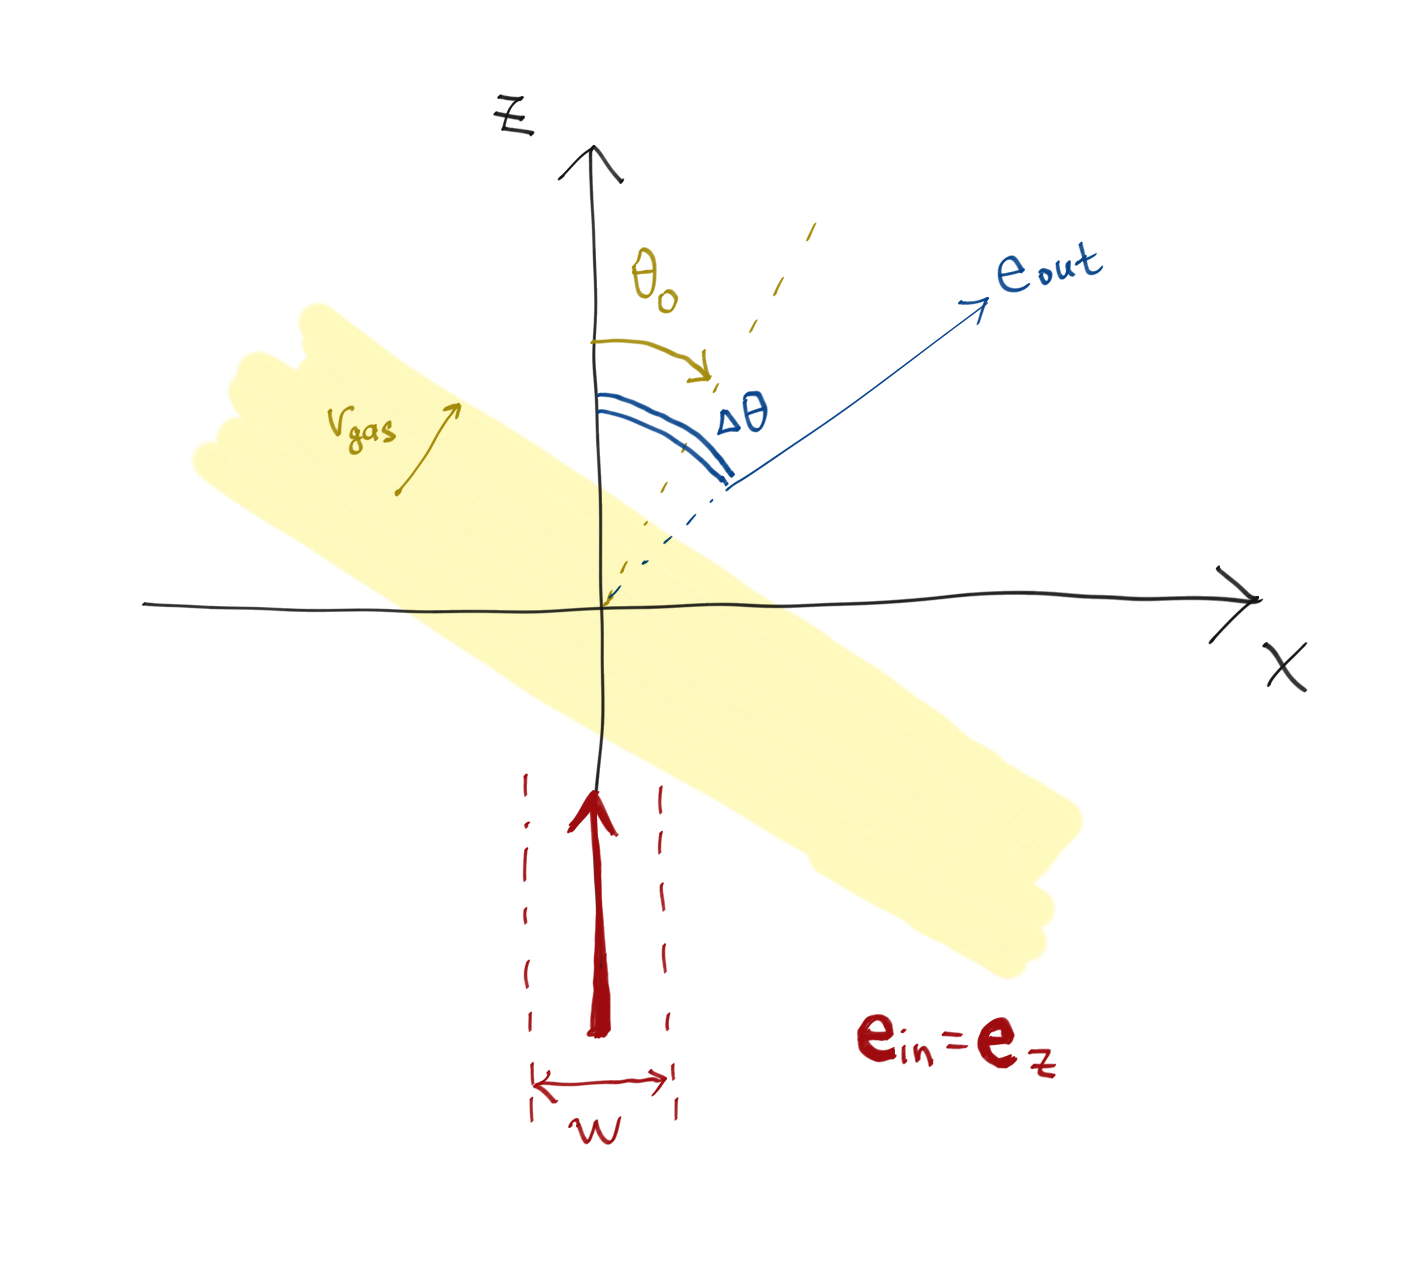
\includegraphics[width=0.43\linewidth]{../img/3ddiffrxzgas}
    }
    \hfil
    \subcaptionbox{$xy$ projection.}{
        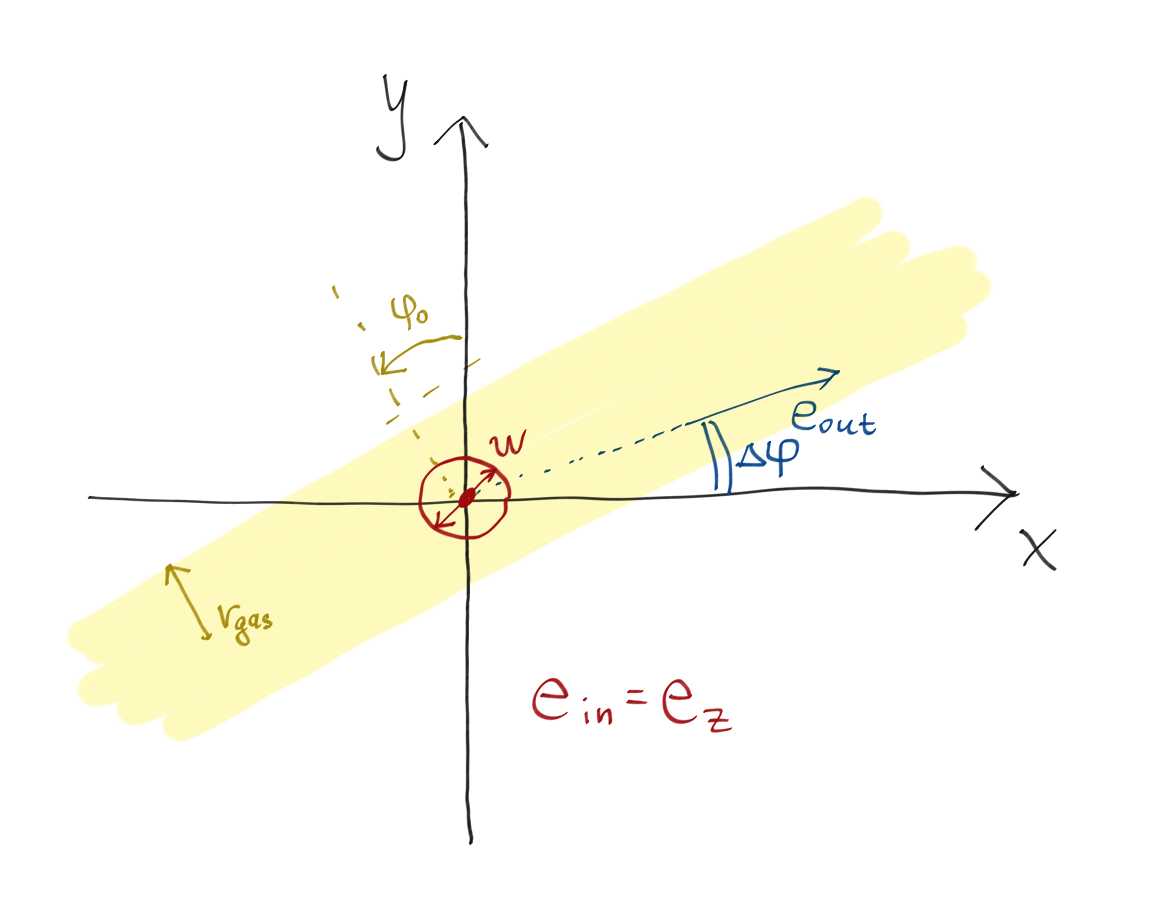
\includegraphics[width=0.43\linewidth]{../img/3ddiffrxygas}
    }
    \label{3ddiffr:image}\caption{General scheme of interaction of incident radiation with a grating. $\theta_0$, $\varphi_0$ --- characterize the target angles in space, $\Delta \theta$, $\Delta \varphi$ --- angles of deflection of the direction of the diffracted radiation relative to the incident, $r_{\textrm{gas }}$ is the radius of the gas jet representing the target, $w$ is the diameter of the Gaussian beam of incident radiation.}
\end{tikzfigure}
        }

        \block[bodyoffsety=1.4cm, titleoffsety=0.7cm]{Monochromatic radiation scattering}{
            \setlength{\parindent}{1em}
            Within the framework of the stationary Mie scattering theory, many clusters were considered in the form of an extended cylindrical gas jet with regular and quasi-regular spatial configuration. The quasi-regular distribution was constructed by introducing random shifts of the coordinates of nodes with an arbitrary shift norm in the range $0 \leq |\Delta d| \leq \eta d$, where $0 \leq \eta < 0.5$ is the degree of irregularity. The program code CELES~\cite{celes} was used for calculations.

\begin{equation}
    E_{\textrm{int}} \left( \eta,\:\lambda, \:V\left(\:\Delta \theta,\:\Delta \varphi \right), \:E_0,\:\varphi_0,\:\theta_0 \right) = \int\limits_{V\left(\:\Delta \theta,\:\Delta \varphi \right)}  |\vectbf{E}{s}\left(\eta,\:\lambda,\:E_0,\:\varphi_0,\:\theta_0\right)|^2 dV,
    \label{e_int}
\end{equation}
\begin{align}
    \vectbf{c}{} = \vectbf{c}{}\left(\vectbf{x}{},\:\Delta \theta,\:\Delta \varphi \right) = M_y(\Delta \theta)\,M_z(\Delta \varphi)\:\vectbf{x}{}, \quad \vectbf{x}{} = \begin{pmatrix}x & y & z\end{pmatrix}^T,
    \label{c_for_e_int}
\end{align}
\begin{align}
    V\left(\:\Delta \theta,\:\Delta \varphi \right) = \left\{\vectbf{x}{} : c_{x}^2 + c_{y}^2 \leq \rho^2, \:\: b_1^2 \leq |\vectbf{x}{}|^2 \leq b_2^2 \right\}.
    \label{V_for_e_int}
\end{align}
        }

        \column{0.33}

        \block{}{
            \setlength{\parindent}{1em}
            \subsubsection{Рассеяние монохроматического излучения}

Для того, чтобы проверить достоверность полученной теории, смоделируем стационарное взаимодействие в регулярном случае при различных параметрах решётки и ширине гауссова пучка $w = 800$ nm, радиусе цилиндра, ограничивающего решетку (радиус газовой струи) $r_{\textrm{gas}} = a + 12d \approx 2$ $\upmu\textrm{m}$, где множитель при $d$ --- количество узлов решетки между центральной осью и границей цилиндра. Несмотря на то, что в реальных условиях гауссов пучок $10$-ой гармоники Ti:Sa лазера с шириной 800 nm получить практически невозможно, в силу стационарности вычислений отношение $w\:/\:r_{\textrm{gas}}$ может быть корректно масштабировано при $w \ll 2r_{\textrm{gas}}$. Использованное малое значение $w$ в таком случае ускоряет вычисления, но принципиально не изменяет их результат.

Различие рассеяния в резонансном и нерезонансном случае показано на \autoref{random_ka0.7:image}: квадрат амплитуды рассеянного поля превышает таковой в отсутствии резонанса более, чем в 10 раз, а также в этом случае нет порядков дифракции, кроме нулевого, что напрямую следует из $\lambda\:/\:d = \lambda_L\:/\:2\lambda_{10} = 5$ в \autoref{bragg_wolf_order_spherical}.

Определим наиболее интенсивные направления рассеяния при помощи следующей интегральной характеристики: %\autoref{1st_check_diffrth:b}:

    \begin{equation}
        E_{\textrm{int}} \left( \eta,\:\lambda, \:V, \:E_0 \right) = \int\limits_{V}  |\vectbf{E}{s}\left(\eta,\:\lambda, \:E_0\right)|^2 dV.
        \label{e_int}
    \end{equation}

В данном случае \autoref{e_int} представляет собой интегрирование интенсивности рассеянного поля, вычисленного как квадрат модуля напряженности рассеянного поля (без учета нормирующего множителя) в области пространства $V$ для решётки, обладающей нерегулярностью $\eta$, то есть является энергией, рассеянной решёткой в область $V$, $\lambda$ представляет собой длину волны падающего поля, $E_0$ --- амплитуду. Область $V$ должна быть задана так, чтобы характеризовать некоторое направление в пространстве, и, как правило, для этой цели используется область в виде конуса, образованного некоторым раствором телесного угла $\delta \Omega$ и направлением при помощи углов $\Delta \theta$, $\Delta \varphi$. Для рассматриваемой задачи необходимо исключить из вычисления ближнее поле, ввиду чего накладывается дополнительное ограничение $V$ внутренностью сферического слоя пространства с границами $b_1$ и $b_2$, где $b_2$ --- граница области численного моделирования, $b_1$ --- больше радиуса сферы, описанной вокруг мишени. Хотя газовая струя является протяженным объектом, в моделировании используется только её сегмент, так как падающий пучок ограничен и рассеяное поле слабо зависит от частей струи, удаленных от области падения пучка, что позволяет описать вокруг такого сегмента соответствующую окружность.

    \img[components/img/eint_scheme]{Схематическое изображение области $V$ (\autoref{V_for_e_int}).}{eint_scheme:image}{0.45\textwidth}

Пересечение конической области и сферического слоя вдали от мишени можно приблизить цилиндром, считая $\rho \approx 0.5\,b_2\cdot\delta \Omega$, где $\rho$ --- радиус цилиндра. В таком случае, при помощи вспомогательного вектора $\vectbf{c}{}$ (\autoref{c_for_e_int}) получаем область $V$ (\autoref{eint_scheme:image}).

    \begin{align}
        \vectbf{c}{} = \vectbf{c}{}\left(x,\:y,\:z,\:\Delta \theta,\:\Delta \varphi \right) = \begin{pmatrix}c_{x}\\c_{y}\\c_{z}\end{pmatrix} = M_y(\Delta \theta)\,M_z(\Delta \varphi)\begin{pmatrix}x\\y\\z\end{pmatrix},
        \label{c_for_e_int}
    \end{align}
    \begin{align}
        V\left(\:\rho, \:b_1, \:b_2, \:\vectbf{c}{} \right) = \left\{\:x,\:y,\:z : c_{x}^2 + c_{y}^2 \leq \rho^2, \:\: b_1^2 \leq x^2 + y^2 + z^2 \leq b_2^2 \right\},
        \label{V_for_e_int}
    \end{align}

\noindentгде $M_y(\Delta \theta)$ --- матрица поворота вокруг декартовой оси $y$ на угол $\Delta\theta$ против часовой стрелки, $M_z(\Delta\varphi)$ --- матрица поворота вокруг декартовой оси $z$ на угол $\Delta\varphi$ против часовой стрелки. В дальнейшем взяты значения $\rho = w\:/\:4$, $b_1 = 4r_{\textrm{gas}}$ где $w$ --- ширина гауссова пучка падающего поля, $r_{\textrm{gas}}$ --- радиус газовой струи, формирующей мишень.

\begin{figure}[H]
    \subimgtwo[components/img/celes/Es_20nm_15deg_1harm.pdf]{$\lambda = \lambda_{L} = 830$ nm.}{random_ka0.7:a}{0.42\textwidth}
    \hfil
    \subimgtwo[components/img/celes/Es_20nm_15deg_10harm.pdf]{ $\lambda = \lambda_{10} = 83$ nm.}{random_ka0.7:b}{0.42\textwidth}
    \caption{$|\vectbf{E}{s}|^2$  в плоскости поляризации, сечение $\Delta \varphi = 0$ --- рассеяние гауссового пучка на слое квазирегулярно расположенных кластеров радиуса $a = 20$ nm, $\theta_0 = 15^{\circ}$, $\varphi_0 = 0^{\circ}$. Границы газового слоя обозначены пурпурным цветом. Амплитуда рассеянного поля нормирована на максимальное значение в случае 10 гармоники.}\label{random_ka0.7:image}
\end{figure}

\begin{figure}[H]
    \subimgtwo[components/img/celes/dphi_dtheta_kprime_d_2l_phi0_0_theta0_15.pdf]{Решение \autoref{bragg_wolf_order_spherical} в целых индексах Миллера.}{1st_check_diffrth:a}{0.335\textwidth}
    \hfil
    \subimgtwo[components/img/celes/e_int_20nm_15deg]{ $E_{\textrm{int}}$ по \autoref{e_int}.}{1st_check_diffrth:b}{0.42\textwidth}
    %\\
    %\subimgtwo[components/img/celes/dphi_dtheta_kprime_d_3l_phi0_0_theta0_15_refr]{$\Delta \theta \in \left[ \cfrac{\pi}{2},\:\pi \right]$.}{1st_check_diffrth:c}{0.27\textwidth}
    %\hfil
    %\subimgtwo[components/img/celes/e_int_cylinder_15edge_theta0_15_phi0_0_249gap_rad50nm_refr]{$\Delta \theta \in \left[ \cfrac{\pi}{2},\:\pi \right]$.}{1st_check_diffrth:d}{0.35\textwidth}
    \caption{Рассеяние 10-ой гармоники при параметрах решетки $a = 20$ nm и $d = 2\lambda_{10}$, $\varphi_0 = 0^{\circ}$, $\theta_0 = 15^{\circ}$, $\lambda = \lambda_{10} = 83$ nm, диапазон построения $\Delta \theta \in \left[ 0,\:\pi\,/\,2 \right]$.}\label{1st_check_diffrth:image}
\end{figure}

Также построим целочисленные решения для $h^\prime,\:k^\prime,\:l^\prime$ с заданными $\theta_0$, $\varphi_0$ в осях $\Delta \varphi$, $\Delta \theta$ при помощи \autoref{bragg_wolf_order_spherical} (\Autoref{1st_check_diffrth:a}). Графики на \autoref{1st_check_diffrth:image} представляют собой диаграммы в полярных координатах $(\Delta \theta, \: \Delta \varphi)$, то есть проекции поверхности сферы, ограниченной некоторым диапазоном угла $\Delta \theta$, на плоскость. Такой метод построения более удобный для изображения пространственного распределения рассеянного излучения, а также более естественный для отображения целочисленных решений на индексы Миллера (\autoref{bragg_wolf_order_spherical}), так как они в таком случае представляют собой наборы колец на сфере. По полученным результатам можно заметить, что наиболее интенсивные направления дифракции по $E_{\textrm{int}}$ отвечают наиболее близкому раположению кривых, соответствующих целочисленным значениям индексов Миллера.

Рассмотрим влияние нерегулярности решетки на наиболее интенсивные направления рассеянного поля, то есть зависимость \autoref{e_int} от нерегулярности решётки $\eta$. Для этого смоделировано рассеяние в случае квазирегулярной решётки при различных параметрах и нерегулярностью $\eta$ от 0 до 0.5 (\Autoref{nonreg_ka0.7:image}).

    % \begin{figure}[H]
    %     \subimgtwo[components/img/celes/e_int_rad_20nm_20deg_nonreg0.0]{$\eta = 0.0$.}{nonreg_mono:a}{0.42\textwidth}
    %     \hfil
    %     \subimgtwo[components/img/celes/e_int_rad_20nm_20deg_nonreg0.1]{$\eta = 0.1$.}{nonreg_mono:b}{0.42\textwidth}
    %     \caption{Характеристика \autoref{e_int} при различной нерегулярности решетки $\eta$, \\$a = 50$ nm, $d = 2\lambda_{10}$, $\varphi_0 = 0^{\circ}$, $\theta_0 = 20^{\circ}$, $\lambda = \lambda_{10} = 83$ nm, диапазон построения $\Delta \theta \in \left[ 0,\:\pi\,/\,2 \right]$.}\label{nonreg_mono:image}
    % \end{figure}

    \begin{figure}[H]

        \subimgtwo[components/img/celes/e_int_20nm_15deg_0.1nonreg.pdf]{$\eta = 0.1$.}{nonreg_ka0.7:b}{0.42\textwidth}
        \hfil
        \subimgtwo[components/img/celes/e_int_20nm_15deg_0.3nonreg]{$\eta = 0.3$.}{nonreg_ka0.7:c}{0.42\textwidth}
        \\
        \subimgtwo[components/img/celes/Es_20nm_15deg_10harm_0.1nonreg.pdf]{$|\vectbf{E}{s}|^2$  в плоскости поляризации, сечение $\Delta \varphi = 0$, $\eta = 0.1$.}{nonreg_ka0.7:a}{0.42\textwidth}
        \caption{Рассеяние гауссового пучка на слое квазирегулярно расположенных кластеров радиуса $a = 20$ nm, $\theta_0 = 15^{\circ}$, $\varphi_0 = 0^{\circ}$.}\label{nonreg_ka0.7:image}
    \end{figure}

    % \begin{figure}[ht]
    %     \subimgtwo[components/img/celes/mean_field_0_42]{Рассеяние $10$-ой гармоники, $\lambda_{10} = 83$ нм, $\eta = 0.43$.}{random_ka0.7:a}{0.4\textwidth}
    %     \hfil
    %     \subimgtwo[components/img/celes/mean_field_0_42_1harm]{Рассеяние лазерной гармоники, $\lambda_{L} = 830$ нм, $\eta = 0.43$.}{random_ka0.7:b}{0.4\textwidth}
    %     \subimgtwo[components/img/celes/reference_regular_14.324]{Рассеяние $10$-ой гармоники, $\lambda_{10} = 83$ нм, $\eta = 0$.}{random_ka0.7:c}{0.4\textwidth}
    %     % \hfil
    %     % \subimgtwo[components/img/celes/check20_rad]{Рассеяние $10$-ой гармоники, $\lambda_{10} = 83$ нм, $|\Delta d|_{\max} = 0$.}{random_ka0.7:c}{0.4\textwidth}
    %     \caption{Рассеяние гауссового пучка ширины $w = 1700$ нм на слое квазирегулярно расположенных кластеров размера $ka = 0.7$ ($a \approx 8.9$ нм), $\theta_0 = 14.32^{\circ}$. Границы газового слоя обозначены пурпурным цветом. Амплитуда $|\vectbf{E}{s}|^2$ построена в плоскости поляризации падающей волны, нормирована на максимальную амплитуду в случае рассеяния 10 гармоники.}\label{random_ka0.7:image}
    % \end{figure}

При помощи нормированного варианта $E_{\textrm{int}}$ (\autoref{e_int_norm}) была построена зависимость изменения рассеяния от нерегулярности решетки (\autoref{energy_vs_nonreg:image}). C ростом нерегулярности решётки наиболее интенсивные направления, кроме нулевого, значительно ослабляются, при этом общая картина рассеяния в различных направлениях выравнивается вплоть до практически однородной при $\eta \to 0.5$ (\autoref{nonreg_ka0.7:image}).

    \begin{equation}
        E_{\textrm{int}}^{\textrm{norm}} \left( \eta,\:\lambda, \:V, \:E_0 \right) = \frac{E_{\textrm{int}} \left( \eta,\:\lambda, \:V, \:E_0 \right)}{E_{\textrm{int}} \left( 0,\:\lambda, \:V, \:E_0 \right)}\label{e_int_norm}
    \end{equation}

    \img[components/img/celes/energy_vs_nonreg]{Ослабление рассеяния в зависимости от нерегулярности решётки.}{energy_vs_nonreg:image}{0.5\textwidth}

Также выявлено ослабление интенсивных направлений рассеяния в зависимости от радиуса кластеров в решётке (\Autoref{radius_wawa:image, energy_vs_radius:image}). При увеличении радиуса кластеров происходит распредление энергии между большим числом направлений (\Autoref{radius_wawa:image}) в соответствии с расположением пересечений кривых, соответствующих целочисленным индексам Миллера (\autoref{1st_check_diffrth:a}), то есть перераспределение в более высокие порядки дифракции по $h^\prime,\:k^\prime,\:l^\prime$. Это связано с уменьшением свободного пространства между узлами решётки при неизменном периоде $d$ --- количество прошедшего излучения уменьшается, расходимость прошедшего через решётку излучения увеличивается, ввиду чего дифракционная картина расплывается, а дифракционные максимумы ослабляются~\cite{born_wolf}.

    \begin{figure}[H]
        \subimgtwo[components/img/celes/e_int_30nm_15deg.pdf]{$a = 30$ nm.}{radius_wawa:a}{0.42\textwidth}
        \hfil
        \subimgtwo[components/img/celes/e_int_60nm_15deg.pdf]{$a = 60$ nm.}{radius_wawa:b}{0.42\textwidth}
        \caption{Характеристика \autoref{e_int} при радиусе кластеров $a = 30$ и $60$ nm, $d = 2\lambda_{10}$, $\varphi_0 = 0^{\circ}$, $\theta_0 = 15^{\circ}$, $\lambda = \lambda_{10} = 83$ nm, диапазон построения $\Delta \theta \in \left[ 0,\:\pi\,/\,2 \right]$.}\label{radius_wawa:image}
    \end{figure}

    \img[components/img/celes/energy_vs_radius]{Ослабление рассеяния в зависимости от радиуса кластеров, значения нормированы на $E_{\textrm{int}}$ при $a = 20$ nm.}{energy_vs_radius:image}{0.5\textwidth}

Была рассмотрена завивимость интенсивных направлений рассеяния по $\Delta \theta$ в зависимости от $\theta_0$ в сечении $\Delta \varphi = 0$. При этом было взято значение $\varphi_0 = 0$, так как любое ненулевое значение этого угла в сути поворачивает угловое распределение на тот же угол, что следует из \autoref{bragg_wolf_order_spherical}.

\begin{comment}
    

% components/img/celes/theta0_dtheta_dphi_phi0_0_miller
    % \img[components/img/celes/theta0_dtheta_dphi_phi0_0.pdf]{Характеристика \autoref{e_int} при различном угле $\theta_0$, $\varphi_0 = 0$, $\Delta \varphi = 0$, $a = 20$ nm, $d = 2\lambda_{10}$.}{dtheta_vs_theta0_eint:image}{0.54\textwidth}

    \begin{figure}[H]
        \subimgtwo[components/img/celes/theta0_dtheta_dphi_phi0_0_miller]{Решение \autoref{bragg_wolf_order_spherical} в целых индексах Миллера.}{theta0_dphi:a}{0.397\textwidth}
        \hfil
        \subimgtwo[components/img/celes/theta0_dtheta_dphi_phi0_0]{$E_{\textrm{int}}$ по \autoref{e_int}.}{theta0_dphi:b}{0.45\textwidth}
        \caption{Рассеяние 10-ой гармоники при различном угле $\theta_0$, $\varphi_0 = 0$, $\Delta \varphi = 0$, $a = 20$ nm, $d = 2\lambda_{10}$. На (а) $k^\prime = 0$ для любых $\theta_0$ и $\Delta \theta$.}\label{theta0_dphi:image}
    \end{figure}

    %\img[components/img/celes/20_rad_1st_check]{Рассеяние гауссового пучка ширины $w = 1700$ нм на слое регулярной решетке кластеров размера $a = 20$ нм, $\theta_0 = 20^{\circ}$. Границы газового слоя обозначены пурпурным цветом. Амплитуда $|\vectbf{E}{s}|^2$ построена в плоскости поляризации падающей волны, нормированая на собственный максимум.}{20rad_1st_check:image}{0.4\textwidth}
\end{comment}
        }

        \block[bodyoffsety=0.7cm]{Wavepacket scattering}{
            \setlength{\parindent}{1em}
            \subsubsection{Рассеяние волнового пакета}

Рассмотрим рассеяние волнового пакета, амплитуда которого описывается гауссовой функцией во времени (\autoref{gaussian_E0}). Рассматривая периодическое продолжение этого импульса на промежутке $[-\tau, \tau]$, где $\tau$ --- ширина импульса, можем построить ряд Фурье (\autoref{gaussian_E0_fourier}). Таким образом, имеем коэффициенты Фурье (\autoref{gaussian_E0_aj}), представляющие собой вклад каждой из гармоник в общий импульс.
%Аппроксимируем такой волновой пакет 10-ой гармоникой, рассмотренной ранее и четырьмя ближайшими к ней, то есть с 8-ой по 12-ую (\autoref{gauss_wavepacket_lambda:image}). 

Для того, чтобы построить диаграмму рассеяния волнового пакета, была использована новая интегральная характеристика, определенная с учетом коэффициентов разложения в ряд Фурье волнового пакета (\autoref{wavepacket_eint}). Такая характеристика разумна для описания направлений рассеяния в силу аддитивности энергии как количественной характеристики. Область $V$ в данном случае представляет собой аналогичную той, что была использована для предыдущей интегральной характеристики (\autoref{V_for_e_int}, \autoref{eint_scheme:image}).

    \begin{equation}
        E_0\left( t \right) = \exp{\left( - \frac{t^2}{\tau^2}\right)}
        \label{gaussian_E0}
    \end{equation}

    \begin{equation}
        E_0\left( t \right) = \frac{\sqrt{\pi}}{2} + \sum_{j = 1}^{\infty}{ a_j \, \cos{\left(\omega_j t \right)}}, \quad \omega_j = \frac{2 \pi j}{\tau} = \frac{c}{\lambda_j}, \quad \lambda_{j} = \frac{\lambda_{L}}{j},
        \label{gaussian_E0_fourier}
    \end{equation}

    \begin{equation}
        a_j = \frac{1}{\tau} \int\limits_{-\tau}^{\tau}  \exp{\left( - \frac{t^2}{\tau^2}\right)} \cos{\left(\omega_j t \right)} dt,
        \label{gaussian_E0_aj}
    \end{equation}

    % \begin{equation}
    %     \vectbf{E}{i} = \sum_{n = 1}^{\infty} E_{0, \: n} \:e^{i n \omega_0 t-ikz}\:\vectbf{e}{x}\label{gaussian_E}
    % \end{equation}

    % \begin{equation}
    %     E_0 \left( \lambda \right) = \frac{1}{\sigma\sqrt{2\pi}}\,e^{-\frac{1}{2}{\left(\frac{\lambda - \mu}{\sigma}\right)}^2}\label{gaussian_E0}
    % \end{equation}

    \begin{equation}
        \EuScript{E}_{\textrm{int}} \left(V, \:\eta\right) = \sum\limits_{j\:=\:N_1\:>\:0}^{N_2}{E_{\textrm{int}} \left( \eta,\:\lambda_{j}, \:V, \:a_j) \right)}
        \label{wavepacket_eint}
    \end{equation}

Определим наиболее интенсивные направления рассеянного поля для решётки с $d = 2\lambda_{10}$, радиусом кластеров $a = 20$~nm, $\theta_0 = 15^\circ$, $\varphi_0 = 0^\circ$, гармоники в волновом пакете с 8-ой по 12-ую, то есть $N_1 = 8$, $N_2 = 12$ в \autoref{wavepacket_eint}, гауссова импульс имеет длину $\tau \approx 17$ fs. 

Сравнивая полученный результат с аналогичной диаграммой, вычисленной при помощи \autoref{e_int} только для 10-ой гармоники, можно заметить значительное усиление нулевого дифракционного максимума ($h^\prime = k^\prime = l^\prime = 0$), отвечающего прошедшему излучению, и небольшое усиление остальных, что полностью соответствует \autoref{bragg_wolf_order_spherical} в силу того, что индексы Миллера, отвечающие дифракционным уравнениям для разных длин волн будут связаны между собой коэффициентами пропорциональности. Таким образом имеем масштабирование кривых, отвечающих целочисленным значениям индексов Миллера.

На \Autoref{wavepacket1:a, wavepacket1:b} видно, что немонохроматичность излучения вносит погрешность для отклонения в заданном направлении --- наиболее интенсивные направления дифракции расплываются (за исключением нулевого).

    % \img[components/img/celes/wavepacket8..12_rad]{Амплитуда элементов гауссова волнового пакета напряженности поля в зависимости от длины волны. Синяя кривая соответствует \autoref{gaussian_E0} с $\mu = 83$~nm, $\sigma = 11$~nm, черные точки --- дискретная аппроксимация волнового пакета, гармоники с 12-ой по 8-ую слева направо.}{gauss_wavepacket_lambda:image}{0.45\textwidth}

    \begin{figure}[ht]
        \subimgtwo[components/img/celes/E_squared/eint_10harm_15deg_0.0nonreg.pdf]{Рассеяние 10-ой гармоники.}{wavepacket1:a}{0.45\textwidth}
        \hfil
        \subimgtwo[components/img/celes/E_squared/eint_wavepacket_15deg_0.0nonreg.pdf]{Рассеяние волнового пакета из гармоник с 8-ой по 12-ую.}{wavepacket1:b}{0.45\textwidth}
        \caption{Полярная диаграмма рассеяния гауссового волнового пакета в сравнении с рассеянием 10-ой гармоники. $\theta_0 = 15^\circ$, $\varphi_0 = 0^\circ$, $d = 2\lambda_{10}$, радиус кластеров $a = 20$ nm.}\label{wavepacket1:image}
    \end{figure}
        }

        \block[bodyoffsety=0.7cm]{Conclusions}{
            \setlength{\parindent}{1em}
            We found that a periodic structure of dense plasma clusters turned out to be a suitable element for efficient directional scattering of radiation in the XUV range. Since many spherical scatterers require calculations in three-dimensional space, a stationary model was proposed and the range of cluster radii was determined, within which the electron density is quasi-stationary during interaction with an external field. When the ionization is such that the electron concentration is close to resonance for given initial parameters, the scattering efficiency increases significantly and reaches several percent in the case of a single cluster. For many clusters, the efficiency of angular dispersion increases with the number of rows of clusters and can reach several percent in the case of certain directions.

The obtained angular distributions of diffraction maxima for scattering by a set of regularly spaced clusters are well described using the Laue theory, while introducing a small irregularity into the distribution of clusters weakens the most intense diffraction directions, which differ from the direction of the transmitted radiation, by no more than 25\%. In the case of non-monochromatic radiation, the efficiency of amplification of the angular dispersion decreases in accordance with the spectral distribution of the field amplitude, the attenuation can reach about three times.
        }

        \block[bodyoffsety=0.7cm]{References}{
            \begin{center}
                \mbox{}\vspace{-1\baselineskip}
                \printbibliography[heading=none] 
            \end{center}
        }

\end{columns}
\end{document}